\section{An interpreter for CRN++}

In the article \textit{CRN++: Molecular Programming Language}, Marko Vasic, David Soloveichik, and Sarfraz Khurshid define a language for programming chemical reactions to perform computation. They define a context-free grammar for this language and explain some of the limitations of the uses and expressiveness of the language when real-world chemical reactions enter the equation. 


\subsection{Grammar}\label{sec:grammar}

Looking at the grammar defined by the article in their listing 1.1, there are immediately some changes we would like to make. Besides this, we impose a few syntactic restrictions to ensure all parsed programs behave as expected. 

In the following, our changes to the grammar is listed. The complete revised grammar can be seen in appendix \ref{sec:grammar_revised}. 

In the article's grammar, it is possible to interchange \texttt{'conc'} and \texttt{'step'} rules, which means a \texttt{'conc'} rule in the bottom of a program could set the concentration of a species used in the beginning. We deemed this unintuitive and in our grammar all \texttt{'conc'} rules must come before all \texttt{'step'} rules. This was done by changing the first rules of the grammar to the following:
\begin{tabbing}
    $\langle \text{Crn} \rangle$ \,::=\; \= \texttt{'crn=\{'$\langle \text{ConcRootSList} \rangle$'\}'} \\
    
    $\langle \text{ConcRootSList} \rangle$ \,::=\;  $\langle \text{ConcS} \rangle$\texttt{','}$\langle \text{ConcRootList} \rangle$ \\
    \>\textbar \, $\langle \text{RootSList} \rangle$ \\

    $\langle \text{RootSList} \rangle$ \,::=\;  $\langle \text{StepS} \rangle$ \\
    \>\textbar \, $\langle \text{StepS} \rangle$\texttt{','}$\langle \text{RootSList} \rangle$
\end{tabbing}
With these rules, a program can have zero or more \texttt{'conc'} statements and at least one \texttt{'step'}. 

In the article's grammar, \texttt{CommandS} includes \texttt{ArithmeticS} nad \texttt{CmpS} but they are not defined. We assume that they refer to the defined but not mentioned \texttt{ModuleS}, since \texttt{ModuleS} contains arithmetic expressions and includes the \texttt{'cmp'} rule. When revising the grammar, we decided to define \texttt{CommandS} as simply each of these, along with \texttt{ConditionalS} which was already a part of it. 

Other than \texttt{ConcS}, there are also other restrictions, all of which we found easier to implement using syntactic restrictions. Firstly, all numbers must be non-negative, since chemical concentrations are always non-negative. Furthermore, to ensure fast and deterministic convergence of all ODEs, there can not be any cycles where one species depends on itself, nor can a species be written to twice in one step. Notice that this implicitly disallows multiple \texttt{cmp} in a single step since all \texttt{cmp} write to the same flags. Lastly, we enforce that all \texttt{ConditionalS} in a step must be mutually exclusive, e.g. \texttt{ifLT} cannot be used together with \texttt{ifLE} since both can be true simultaneously. Additionally, there can not be any nested \texttt{if}. This does not reduce expressiveness of the language and makes it simpler to check the restrictions. 

In short, our syntactic restrictions are:
\begin{enumerate}
    \item All numbers must be non-negative
    \item No species may be written to more than once in a single step
    \item Species may not write to each other in a cyclic fashion
    \item If branches must be mutually exclusive
    \item There can be no nested if statements
\end{enumerate}


\subsection{Abstract syntax tree (AST)}
Having a grammar suitable for our needs, we can now define F\# types that comprise our model for the abstract syntax tree used for the compiler. These type declarations are given as follows. 

The AST is rooted in Root: 
\begin{minted}{haskell}
    type Root = R of Conc List * Step List
\end{minted}
which forces all concentration definitions to come before the steps, where Conc is defined as:
\begin{minted}{haskell}
    type Conc = C of species * float
\end{minted}
Each step is comprised of a list of \texttt{Commands} like so
\begin{minted}{haskell}
    type Step = S of Command List
\end{minted}
Where the definition of \texttt{Command} is:
\begin{minted}{haskell}
    type Command =
        | Ld of species * species
        | Add of species * species * species
        | Sub of species * species * species
        | Mul of species * species * species
        | Div of species * species * species
        | Sqrt of species * species
        | Cmp of species * species
        | Rx of species List * species List * float
        | IfGT of Command List
        | IfGE of Command List
        | IfEQ of Command List
        | IfLT of Command List
        | IfLE of Command List
\end{minted}
And \texttt{species} is just a string, that signifies the name of the species:
\begin{minted}{haskell}
    type species = string
\end{minted}

Using this structure for the AST, the \texttt{integer square root} program can be visualized as seen in figure \ref{fig:ast_sqrt}, using our tree code from project 1.  

\begin{figure}[ht!]
    \centering
    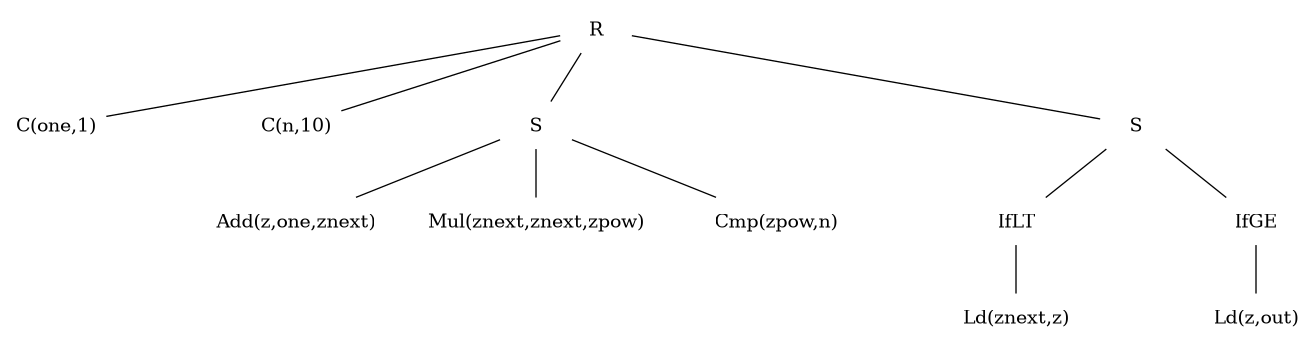
\includegraphics[width=\textwidth]{report/figures/ast_sqrt.png}
    \caption{AST for the integer square root program}
    \label{fig:ast_sqrt}
\end{figure}


\subsection{Parser}

In order to write CRN++ programs and compile them to chemical reactions, a parser was developed using \texttt{FParsec}. We will not go into much detail as to how this was implemented but simply cover the main decisions we took during the development of the parser. Firstly we realized that white space had no effect in the CRN++ language. Therefore we chose to simply remove all white space from an input string before parsing. This made working with \texttt{FParsec} much easier. The parser essentially follows our revised grammar but with the modification that there can be no nested if statements. Nested if statements is allowed by the grammar but is not allowed by our language. We discovered that not allowing nested if statements made parsing far easier and therefore we simply implemented it here instead of in the type checker.



\subsection{Type checker}
After parsing a program, we have an AST. However, this AST might not be well-formed, i.e. follow the four rules extraneous to the grammar detailed in section \ref{sec:grammar}. This is where the type checker comes in. 

The first rule, that all numbers must be non-negative, is only relevant for the \texttt{conc} statements and is therefore checked in the beginning. Afterwards, each of the remaining three rules are concerned only with the content of a single step in a program and steps can therefore be type checked independently of each other. By recursively matching on each step in the \texttt{StepList} in the AST, the type checker maintains the following accumulating values: a set of species which have been written to doing this step, a set of which if-statements have been used this step, as well as a certain graph $G$. The nodes of $G$ represent species and an edge from $a\to b$ signals that $a$ is input to $b$. By then trying to topologically sort $G$, we can quickly check if $G$ is a $DAG$ and thereby does not contain any cycles.



\subsection{State and interpreter}
The state recording the concentration of each species is simply a map from each species to its corresponding value. Its declaration in F\# is:
\begin{minted}{haskell}
    type State = Map<species, float>
\end{minted}
Since each \texttt{State} only depends on the last \texttt{State} and the steps, one can make an infinite \texttt{State} sequence by implementing a function that generates the next state based on the current state:
\begin{minted}{haskell}
    let doStep (S(cl): Step) (state: State) : State = doCommandList cl state
\end{minted}
and utilizing it in an unfold. The interpret function then becomes:
\begin{minted}{haskell}
    let interpretProgram (R(concl, stepl)) (initialState: State) =
        if not (isTyped (R(concl, stepl))) then
            failwith "Does not typecheck"
        else
            Seq.unfold
                (fun (state, i) ->
                    let nextState = doStep (List.item (i % List.length stepl) stepl)
                        state Some(nextState, (nextState, i + 1)))
                (initialState, 0)
\end{minted}

This is supplied with the function \texttt{getInitialState} which reads all the initial concentrations:
\begin{minted}{haskell}
    let getInitialState (concl: Conc List) : State =
        List.fold (fun state (C(s, c)) -> Map.add s c state) Map.empty concl
\end{minted}


\subsection{Testing}
We wanted to use property based testing, in the hope that it would be as applicable here as it was when drawing trees in the first project. However, there were some obstacles. It was not easy to get \texttt{FsCheck} to generate an AST that could have resulted from a valid parsed program. Furthermore, generating programs and then parsing them was also not doable, since the fraction of valid programs over invalid programs is vanishingly small. Thus we opted for a more traditional approach to testing, where we have programs that we know are correct and programs that we know are flawed, and we make tests on these. \texttt{FsCheck} then picks one of these programs and we check that mapping shuffle on each \texttt{StepList} does not change whether it type checks or the resulting sequence of states. Since one cannot compare infinite sequences directly, we only check whether the first 50 steps match.

To increase the coverage of the tests, all the operators from Table 1 in the paper were tested in isolation, where \texttt{FsCheck} picks for example the numbers to add. These were then compared to the result from the same operations in \texttt{F\#}.


We expected that all tests would pass, however, we found that the ordering inside a step influences the result. As we will cover in the assessment, we found that this is not a mistake, but a fault in the problem description.

\subsection{Visualization}
To visualize the sequence of states, we first output the sequence to a file, in a manner where we can easily read it into Python.

We then load this into Python and get a list of all the species, and a matrix where row $i$ corresponds to the state in step $i$. The $j$th index in all rows refers to the concentration of the $j$th species, therefore, by transposing the matrix, the $i$th row becomes the data points that are to be plotted for species $i$. By then having two copies of each value except the last value, and having the x-axis $0,0.99,1,1.99,2,2.99\dots$ instead of $0,1,2\dots$ we get the stair plot that clearly shows the step-wise process instead of a continuous progression between steps.

To make the plots a bit nicer and easier to read, the lines have different opaque colours and one can elect which species are plotted through command line arguments. Every CRN program from the article has been interpreted, plotted and can be found in appendix \ref{sec:interpreter_plots}. 

\subsection{Assessment}
Making an interpreter for the CRN language which behaves like the chemical reactions it models is for the most part simple. The few modules that have to be implemented are arithmetic operations and the logic for if-statements. However, one issue rises above all: the order in which to execute the operations within each step. 

\subsubsection{On the parallel execution of steps}
In the chemical reactions that we model, every module (and therefore reaction) in a step happens simultaneously. Does this mean, then, that we should simply update the state by saving each previous value, calculate the new values for each species using only the old values and then update the state for the next step? No, because some chemical reactions depend on each other. Consider the following example of the integer square root CRN++ program from the article:
\begin{verbatim}
crn = {
    conc[one,1],conc[n,10],
    step[{
        add[z,one,znext],
        mul[znext,znext,zpow],
        cmp[zpow,n]
    }],
    ...  // omitted to save space
\end{verbatim}

Notice that in this step, \texttt{znext} is both written to and used for another reaction, where \texttt{zpow} is written to and then also used in a comparison. When simulating the chemical reactions for this, all of these steps are calculated at the same time, and they converge to the values that we expect. However, for this program to be interpreted in the same way, the order of execution matters. Recall that we require a well-formed program to avoid cyclic dependencies within steps. This means that it is possible to order the executions within each step according to a topological sorting, and it is clear to see that this is actually the only correct way to execute the steps in order to model the same behavior as the chemical reactions. Otherwise, the wrong values for certain species would be used in the calculations, since they could be used before they were written to in a step. 

\subsubsection{Our implementation}
While we are proud of the above analysis, we discovered this fact late in the project and thus did not have enough time to implement it in the interpreter. In summary, our current interpreter executes each module in a step in a top-to-bottom manner, updating the concentration of each species along the way. This means that it interprets CRN programs correctly if the modules within each step already satisfy a topological ordering, such as the integer square root example does. 

We would have liked to implement a topological sorting in the interpreter, just like we did in the type checker, given more time. 
